% Tinplate Reverb - manuel d'utilisation.
% pdflatex manuel.tex (trois passes) ; figures : python3 figures.py (doc/fig_*.pdf).
% Copyright (C) 2026 Tinplate authors - SPDX-License-Identifier: GPL-3.0-or-later
\documentclass[a4paper,11pt]{article}
\usepackage[T1]{fontenc}
\usepackage[utf8]{inputenc}
\usepackage[french]{babel}
\usepackage{lmodern}
\usepackage{microtype}
\usepackage[margin=2.3cm]{geometry}
\usepackage{amsmath,amssymb}
\usepackage{graphicx}
\usepackage{booktabs}
\usepackage{array}
\usepackage{tabularx}
\usepackage{xcolor}
\usepackage{tikz}
\usetikzlibrary{arrows.meta,positioning,fit,calc}
\usepackage{enumitem}
\usepackage[hidelinks]{hyperref}

\definecolor{brass}{HTML}{966919}
\definecolor{steel}{HTML}{196E96}
\definecolor{ink}{HTML}{1E262D}
\definecolor{paper}{HTML}{F2F5F7}

\newcommand{\ctl}[1]{\textsf{\textbf{#1}}}   % nom d'un élément de l'interface
\newcommand{\dB}{\,dB}
\newcommand{\dBFS}{\,dBFS}
\setlist{itemsep=1pt,topsep=3pt}
\emergencystretch=3em
\graphicspath{{./}{captures/}}

\title{\textcolor{steel}{\textbf{TINPLATE}} \textsf{REVERB}\\[4pt]
\large Manuel d'utilisation et description de l'algorithme}
\author{Version 1.0.0}
\date{}

\begin{document}
\maketitle

\begin{center}
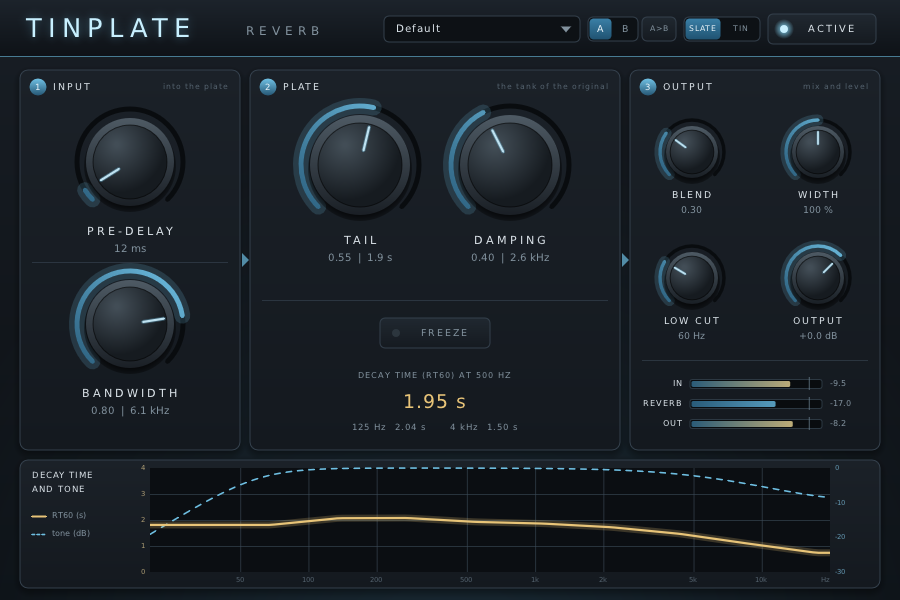
\includegraphics[width=0.92\textwidth]{capture_interface.png}
\end{center}

\newpage
\tableofcontents
\newpage

% ==============================================================================================
\section{Présentation}

Tinplate Reverb est une réverbération à plaque. Son cœur est celui de \texttt{PlateX2} de CAPS,
la bibliothèque de greffons LADSPA de Tim Goetze (appelé \texttt{Plate2x2} dans la série 0.4),
lui-même construit sur la plaque décrite par Jon Dattorro (\emph{Effect Design, Part 1},
J. Audio Eng. Soc., 1997). Ce cœur est repris à l'identique, opération par opération : avec les
ajouts au neutre, la sortie est celle de l'original au bit près (section~\ref{sec:identite}).

Autour de ce cœur, Tinplate ajoute ce qui manque pour un usage courant : pré-retard, coupe-bas
sur la réverbération, largeur stéréo, gel (\emph{Freeze}), gain de sortie, lissage des réglages,
affichage du temps de réverbération réel, préréglages, comparaison A/B.

\paragraph{Formats.} VST3 et CLAP pour Windows 64 bits ; VST3, CLAP et LV2 pour Linux. Le greffon
est stéréo (deux entrées, deux sorties) ; sa latence est nulle.

\paragraph{Licence.} GPL 3 ou ultérieure, comme CAPS (fichier \texttt{COPYING}). L'interface et
l'adaptation aux formats reposent sur DPF (licence ISC).

% ==============================================================================================
\section{Installation}

\paragraph{Windows.} Lancer \texttt{Tinplate-Reverb-1.0.0-setup.exe} : il installe le VST3
(obligatoire) et, si on le coche, le CLAP et ce manuel, puis ajoute un désinstalleur
(\og Programmes et fonctionnalités\fg). À la main : copier le dossier
\texttt{tinplate\_reverb.vst3} dans \verb|C:\Program Files\Common Files\VST3\| et
\texttt{tinplate\_reverb.clap} dans \verb|C:\Program Files\Common Files\CLAP\|.

\paragraph{Linux.} Copier \texttt{tinplate\_reverb.vst3} dans \verb|~/.vst3/|,
\texttt{tinplate\_reverb.clap} dans \verb|~/.clap/| ou \texttt{tinplate\_reverb.lv2} dans
\verb|~/.lv2/|.

Relancer ensuite l'analyse des greffons de l'hôte. Le désinstalleur laisse les préférences et
les préréglages de l'utilisateur (section~\ref{sec:fichiers}).

% ==============================================================================================
\section{Prise en main en une minute}

\begin{enumerate}
\item \textbf{En insert} sur une piste : le préréglage \ctl{Default} est chargé (Blend 0,30,
  réverbération d'environ 1,9\,s à 500\,Hz). \textbf{En départ auxiliaire} : choisir
  \ctl{Send (100 \% wet)}, qui ne rend que la réverbération.
\item Régler la longueur avec \ctl{TAIL} ; la valeur en secondes s'affiche sous le bouton et au
  centre de la section 2.
\item Assombrir ou éclaircir avec \ctl{DAMPING} (aigus qui meurent plus vite dans la queue) et
  \ctl{BANDWIDTH} (aigus qui entrent dans la plaque).
\item Éloigner la réverbération du son direct avec \ctl{PRE-DELAY} (20 à 40\,ms sur une voix) ;
  nettoyer le grave du mixage avec \ctl{LOW CUT}.
\item Doser avec \ctl{BLEND}. \ctl{FREEZE} tient la réverbération indéfiniment.
\end{enumerate}

% ==============================================================================================
\section{L'interface}

La fenêtre (900 × 600 points, redimensionnable en gardant ses proportions, nette sur les écrans à
haute densité) se lit de gauche à droite dans l'ordre du signal : trois sections numérotées
reliées par des flèches, puis le graphique du temps de réverbération en bas. Chaque élément a une
bulle d'aide au survol ; pour un bouton, son titre donne la valeur détaillée.

\begin{center}
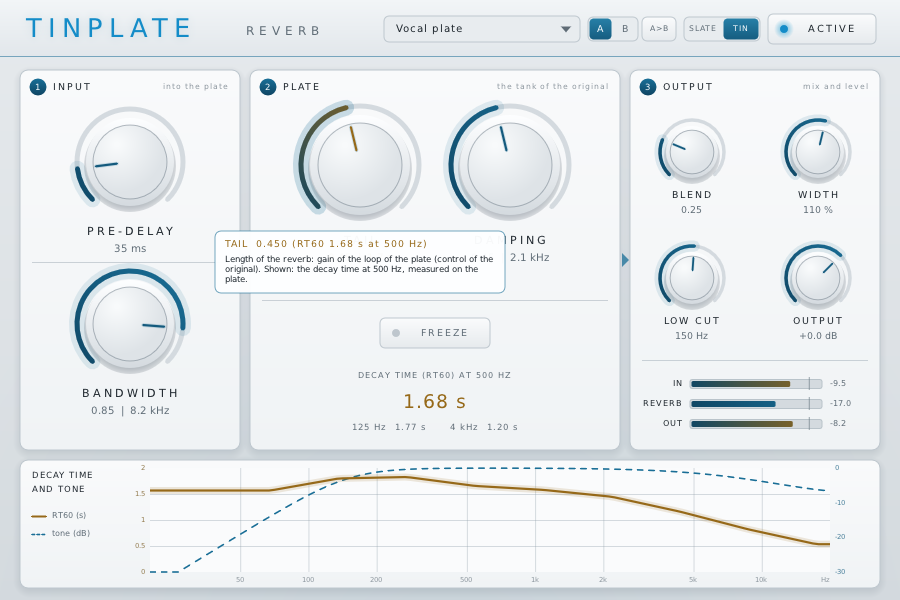
\includegraphics[width=0.8\textwidth]{capture_interface_tin.png}\\[2pt]
\small Thème clair \ctl{TIN}, bulle d'aide de Tail.
\end{center}

\subsection{En-tête}
\begin{description}
\item[Préréglages.] Liste déroulante : un clic l'ouvre ; elle montre les préréglages d'usine
  (\ctl{FACTORY}), un trait, vos préréglages (\ctl{USER}, par ordre alphabétique), un trait, puis
  \ctl{Save current settings\ldots}. Le préréglage courant est marqué d'un point ; \og *\fg{}
  après son nom signale un réglage modifié depuis son chargement. La molette sur la boîte fermée
  passe au préréglage suivant ou précédent. Détails en section~\ref{sec:prereglages}.
\item[A | B et A>B.] Deux jeux de réglages à comparer : un clic sur \ctl{A} ou \ctl{B} bascule
  (le jeu quitté est gardé, l'autre est rechargé ; à la première visite, B part d'une copie de
  A). \ctl{A>B} (ou \ctl{B>A}) copie le jeu courant dans l'autre. Les deux jeux sont
  enregistrés avec le projet.
\item[SLATE | TIN.] Thème sombre ou clair, sans effet sur le son ; c'est une préférence de
  l'ordinateur, commune à toutes les instances et à tous les projets.
\item[ACTIVE / BYPASSED.] Le Bypass déclaré à l'hôte (section~\ref{sec:lissage}).
\end{description}

\subsection{Section 1 : INPUT}
\ctl{PRE-DELAY} et \ctl{BANDWIDTH} : ce qui entre dans la plaque. Sous Bandwidth, sa valeur et
la fréquence à $-3$\dB{} du filtre à la fréquence d'échantillonnage courante (\og open\fg{}
quand il reste au-dessus de $-3$\dB{} jusqu'à la fréquence de Nyquist).

\subsection{Section 2 : PLATE}
\ctl{TAIL} et \ctl{DAMPING}, les deux grands boutons de la boucle ; sous Damping, la fréquence à
$-3$\dB{} de son filtre. Au centre, le temps de réverbération (RT60) à 500\,Hz, en grand, et à
125\,Hz et 4\,kHz. Le bouton \ctl{FREEZE} gèle la réverbération ; Tail et Damping sont alors
grisés, puisqu'ils n'agissent plus.

\subsection{Section 3 : OUTPUT}
\ctl{BLEND}, \ctl{WIDTH}, \ctl{LOW CUT}, \ctl{OUTPUT}, puis trois vu-mètres de crête :
\ctl{IN} (entrée), \ctl{REVERB} (réverbération seule, après Low cut et Width, avant le
mélange), \ctl{OUT} (sortie), en dBFS ; après une crête, l'affichage redescend avec une constante de temps de 0,25\,s.

\subsection{Temps de réverbération et tonalité}
En bas, sur une échelle de fréquences de 20\,Hz à 20\,kHz (ou à la fréquence de Nyquist) :
\begin{itemize}
\item en laiton, le \textbf{temps de réverbération} en fonction de la fréquence (échelle de
  gauche, en secondes ; pleine échelle de 2, 4, 6 ou 8\,s selon la courbe), réglé par Tail et
  Damping ; pendant le gel, la mention \og FROZEN: infinite decay\fg ;
\item en acier et en tirets, la \textbf{tonalité} de la réverbération (échelle de droite, en
  dB), réglée par Bandwidth et Low cut.
\end{itemize}

\subsection{Manipuler les boutons}
\begin{itemize}
\item glisser verticalement ; \textsf{Maj} pour un réglage fin ;
\item molette (\textsf{Maj} : fin) ;
\item double-clic ou \textsf{Ctrl}+clic : valeur par défaut ;
\item clic droit : saisie de la valeur au clavier (\textsf{Entrée} valide, \textsf{Échap}
  annule ; la virgule est acceptée comme séparateur décimal).
\end{itemize}

% ==============================================================================================
\section{Les réglages}

\begin{center}
\small
\begin{tabularx}{\textwidth}{@{}l l l X@{}}
\toprule
Réglage & Plage & Défaut & Rôle \\
\midrule
Pre-delay & 0--250\,ms & 0\,ms & retard avant la plaque \\
Bandwidth & 0--1 & 0,5 & passe-bas d'entrée de la plaque (original) \\
Tail & 0--1 & 0,5 & longueur de la réverbération (original) \\
Damping & 0--1 & 0,75 & passe-bas dans la boucle (original) \\
Freeze & oui/non & non & réverbération tenue sans fin \\
Blend & 0--1 & 0,25 & part du signal traité (original) ; 1 : réverbération seule \\
Width & 0--200\,\% & 100\,\% & largeur stéréo de la réverbération \\
Low cut & 20\,Hz (off)--1\,kHz & off & passe-haut 12\dB/octave sur la réverbération seule \\
Output & $-24$--+12\dB & 0\dB & gain de toute la sortie \\
Bypass & oui/non & non & entrée non traitée, fondu de 10\,ms \\
\bottomrule
\end{tabularx}
\end{center}
Les défauts des quatre réglages de l'original (Bandwidth, Tail, Damping, Blend) sont ceux qu'un
hôte LADSPA donne à PlateX2 ; le préréglage \ctl{Default}, chargé à l'ouverture, est différent
(section~\ref{sec:prereglages}).

\paragraph{Pre-delay.} Retarde l'entrée de la plaque : la réverbération démarre plus tard que le
son direct, qui reste plus lisible (voix, caisse claire). Le son sec n'est pas retardé. Un
changement passe de l'ancien retard au nouveau par un fondu enchaîné de 30\,ms : pas de
glissement de hauteur ni de clic.

\paragraph{Bandwidth.} Passe-bas du premier ordre à l'entrée de la plaque : il règle la part
d'aigus qui y entre, donc la brillance de toute la réverbération, attaque comprise. Il n'agit
pas sur la durée.

\paragraph{Tail.} Gain de la boucle de la plaque : plus il est grand, plus la réverbération est
longue (de 0,6 à 5,1\,s à 500\,Hz ; figure~\ref{fig:rt60}). Même à 0, la plaque
résonne environ 0,6\,s : ses filtres passe-tout sonnent d'eux-mêmes.

\paragraph{Damping.} Passe-bas du premier ordre dans la boucle : à chaque tour, les aigus perdent
un peu plus que les graves, si bien qu'ils s'éteignent plus tôt (son plus sombre, plus
naturel). À 0, la boucle n'amortit pas les aigus.

\paragraph{Freeze.} La plaque cesse de recevoir le signal et de perdre son énergie : la
réverbération en cours est tenue indéfiniment, au même niveau et avec le même timbre. On peut
jouer par-dessus : le signal sec passe toujours, mais ce qui est joué pendant le gel n'entre
pas dans la plaque. En le relâchant, la réverbération reprend sa décroissance selon Tail et
Damping. Détails en section~\ref{sec:freeze}.

\paragraph{Blend.} Mélange du sec et du traité, avec la loi de l'original : traité $=
\mathrm{blend}^{1{,}53}$, sec $= 1 - \text{traité}$ (figure~\ref{fig:lois}). À 0,25, la
réverbération est à $-18{,}4$\dB{} et le sec à $-1{,}1$\dB ; à 1, il ne reste que la
réverbération (départ auxiliaire).

\paragraph{Width.} Largeur stéréo de la réverbération seule : 0\,\% la rend mono, 100\,\% la
laisse telle quelle, 200\,\% double la différence entre les canaux. Le sec n'est pas touché.

\paragraph{Low cut.} Passe-haut de Butterworth du second ordre (12\dB{} par octave) sur la
réverbération seule : il retire le grave qui brouille le bas du mixage sans toucher au son sec.
Le bouton est logarithmique ; à son minimum (20\,Hz, \og off\fg), le filtre est retiré.

\paragraph{Output.} Gain de la sortie entière (sec et traité), après le mélange.

% ==============================================================================================
\section{Préréglages}\label{sec:prereglages}

\subsection{Préréglages d'usine}
\begin{center}
\small
\begin{tabular}{@{}l r r r r r r r r@{}}
\toprule
Nom & Bandw. & Tail & Damp. & Blend & Pre-d. & Low cut & Width & RT60 \\
\midrule
Default           & 0,80 & 0,55 & 0,40 & 0,30 & 12 & 60  & 100 & 1,9 \\
Original (CAPS)   & 0,50 & 0,50 & 0,75 & 0,25 & 0  & off & 100 & 1,6 \\
Vocal plate       & 0,85 & 0,45 & 0,45 & 0,25 & 35 & 150 & 110 & 1,7 \\
Drum plate        & 0,90 & 0,30 & 0,30 & 0,22 & 5  & 200 & 120 & 1,3 \\
Ambience          & 0,70 & 0,15 & 0,50 & 0,20 & 0  & 100 & 130 & 0,9 \\
Dark and long     & 0,55 & 0,85 & 0,75 & 0,35 & 20 & 60  & 100 & 2,9 \\
Bright and wide   & 1,00 & 0,70 & 0,10 & 0,30 & 15 & 120 & 150 & 2,6 \\
Send (100 \% wet) & 0,80 & 0,60 & 0,40 & 1,00 & 20 & 100 & 100 & 2,1 \\
\bottomrule
\end{tabular}
\end{center}
Pre-delay en ms, Low cut en Hz, Width en \%, RT60 à 500\,Hz en secondes (à 44,1\,kHz) ; Output à
0\dB{} partout, Freeze inactif. \og Original (CAPS)\fg{} reproduit l'original au bit près. Ces
préréglages ont été réglés d'après les lois des réglages, pas à l'oreille. Ils sont aussi
présentés à l'hôte (liste des programmes).

\subsection{Vos préréglages}
\begin{description}
\item[Enregistrer.] Dans la liste, \ctl{Save current settings\ldots}, puis taper le nom
  directement dans la boîte (proposé : le nom de votre préréglage en cours). \textsf{Entrée}
  enregistre, \textsf{Échap} ou un clic ailleurs annule. Une bulle dit ce que fera
  \textsf{Entrée} : enregistrer, remplacer votre préréglage du même nom (majuscules et minuscules
  confondues), ou refuser : nom d'un préréglage d'usine, nom invalide, dossier non inscriptible.
  Noms : 1 à 24 caractères ASCII imprimables, sans \verb|< > : " / \ | ? *|, sans espace ni point
  au début ou à la fin, ni nom réservé de Windows (\texttt{CON}, \texttt{NUL}\ldots).
\item[Supprimer.] Survoler votre préréglage dans la liste : une croix apparaît à droite. Un
  premier clic affiche \og delete?\fg, un second supprime (sans retour en arrière).
\item[Portée.] Vos préréglages sont communs à tous les projets, toutes les instances et tous les
  hôtes de l'ordinateur ; la liste est relue à chaque ouverture, le fichier à chaque chargement.
  L'hôte, lui, ne voit que les préréglages d'usine ; ses propres préréglages (par exemple
  \texttt{.vstpreset}) restent possibles et indépendants.
\end{description}
Freeze et Bypass, qui servent au jeu et à l'écoute, ne font partie d'aucun préréglage ni du jeu
A/B.

% ==============================================================================================
\section{L'algorithme}

Cette section décrit exactement le calcul fait par le greffon (fichiers
\nolinkurl{plugin/TinplatePlugin.cpp} et \nolinkurl{plugin/PlateCore.hpp}). Les figures sont
calculées avec les mêmes formules et, pour les réponses impulsionnelles, avec le code de la plaque
lui-même.

\subsection{Chaîne du signal}

\begin{center}
\begin{tikzpicture}[
  node distance=4mm and 4mm,
  blk/.style={draw=ink, rounded corners=2pt, fill=paper, minimum height=7mm, align=center,
              font=\footnotesize\sffamily, inner sep=3pt},
  core/.style={blk, fill=brass!15, draw=brass},
  arr/.style={-{Stealth[length=2mm]}, ink}]
\node[blk] (in) {entrée\\$L, R$};
\node[blk, right=of in] (sum) {$(L+R)/2$};
\node[blk, right=of sum] (pre) {Pre-delay};
\node[blk, right=of pre] (frz) {× entrée\\(Freeze)};
\node[core, right=of frz] (plate) {plaque\\(original)};
\node[blk, below=10mm of plate] (lc) {Low cut};
\node[blk, left=of lc] (wd) {Width};
\node[blk, left=of wd] (mix) {mélange\\Blend};
\node[blk, left=of mix] (out) {Output};
\node[blk, left=of out] (byp) {Bypass\\(fondu)};
\node[blk, below=8mm of byp] (s) {sortie};
\draw[arr] (in) -- (sum); \draw[arr] (sum) -- (pre); \draw[arr] (pre) -- (frz);
\draw[arr] (frz) -- (plate); \draw[arr] (plate) -- node[right, font=\scriptsize] {$w_L, w_R$} (lc);
\draw[arr] (lc) -- (wd); \draw[arr] (wd) -- (mix);
\draw[arr] (mix) -- (out); \draw[arr] (out) -- (byp); \draw[arr] (byp) -- (s);
\draw[arr, dashed] (in.south) -- ++(0,-4mm) -| node[pos=0.3, above, font=\scriptsize] {signal sec} (mix.north);
\draw[arr, dashed] (in.west) -- ++(-4mm,0) |- node[pos=0.25, left, font=\scriptsize] {entrée} (byp.west);
\end{tikzpicture}
\end{center}

L'entrée stéréo est ramenée en mono, comme dans l'original, avec une constante de $\pm10^{-20}$
($-400$\dB, signe alterné à chaque échantillon) qui tient la plaque hors des nombres dénormaux ;
la plaque rend deux canaux, $w_L$ et $w_R$. Tout le reste est stéréo.

\subsection{La plaque}\label{sec:plaque}

\begin{center}
\begin{tikzpicture}[
  node distance=3mm and 3mm,
  blk/.style={draw=ink, rounded corners=2pt, fill=paper, minimum height=6.5mm, align=center,
              font=\scriptsize\sffamily, inner sep=2pt},
  ap/.style={blk, fill=steel!12, draw=steel},
  lp/.style={blk, fill=brass!15, draw=brass},
  arr/.style={-{Stealth[length=1.6mm]}, ink}]
\node[blk] (x) {$x$};
\node[lp, right=of x] (bw) {passe-bas\\Bandwidth};
\node[ap, right=of bw] (d1) {passe-tout\\4,8\,ms};
\node[ap, right=of d1] (d2) {passe-tout\\3,6\,ms};
\node[ap, right=of d2] (d3) {passe-tout\\12,7\,ms};
\node[ap, right=of d3] (d4) {passe-tout\\9,3\,ms};
\node[circle, draw=ink, inner sep=1pt, font=\scriptsize, below=8mm of d1] (sL) {$+$};
\node[ap, right=of sL] (mL) {passe-tout\\modulé 22,6\,ms};
\node[blk, right=of mL] (tL) {retard\\149,6\,ms};
\node[lp, right=of tL] (dL) {passe-bas\\Damping};
\node[blk, right=of dL] (gL) {× decay};
\node[ap, right=of gL] (aL) {passe-tout\\60,5\,ms};
\node[blk, right=of aL] (uL) {retard\\125,0\,ms};
\node[blk, right=of uL] (hL) {× decay};
\node[circle, draw=ink, inner sep=1pt, font=\scriptsize, below=10mm of sL] (sR) {$+$};
\node[ap, right=of sR] (mR) {passe-tout\\modulé 30,5\,ms};
\node[blk, right=of mR] (tR) {retard\\141,7\,ms};
\node[lp, right=of tR] (dR) {passe-bas\\Damping};
\node[blk, right=of dR] (gR) {× decay};
\node[ap, right=of gR] (aR) {passe-tout\\89,2\,ms};
\node[blk, right=of aR] (uR) {retard\\106,3\,ms};
\node[blk, right=of uR] (hR) {× decay};
\draw[arr] (x) -- (bw); \draw[arr] (bw) -- (d1); \draw[arr] (d1) -- (d2); \draw[arr] (d2) -- (d3);
\draw[arr] (d3) -- (d4);
\draw[arr] (d4.south) -- ++(0,-3mm) -| ($(sL.west)+(-4mm,0)$) -- (sL.west);
\draw[arr] ($(sL.west)+(-4mm,0)$) |- (sR.west);
\draw[arr] (sL) -- (mL); \draw[arr] (mL) -- (tL); \draw[arr] (tL) -- (dL); \draw[arr] (dL) -- (gL);
\draw[arr] (gL) -- (aL); \draw[arr] (aL) -- (uL); \draw[arr] (uL) -- (hL);
\draw[arr] (sR) -- (mR); \draw[arr] (mR) -- (tR); \draw[arr] (tR) -- (dR); \draw[arr] (dR) -- (gR);
\draw[arr] (gR) -- (aR); \draw[arr] (aR) -- (uR); \draw[arr] (uR) -- (hR);
\draw[arr] (hL.south) -- ++(0,-2.5mm) -| (sR.north);
\draw[arr] (hR.east) -- ++(3mm,0) |- ($(sL.north)+(0,2.5mm)$) -- (sL.north);
\end{tikzpicture}
\end{center}

\paragraph{Diffusion d'entrée.} Après le passe-bas Bandwidth, quatre filtres passe-tout en
série (coefficients 0,742, 0,742, 0,712, 0,712) dispersent l'impulsion en un nuage d'échos
denses avant la boucle.

\paragraph{Réservoir.} Deux moitiés croisées : la sortie de chaque moitié, multipliée par
$\mathrm{decay}$, s'ajoute à l'entrée de l'autre. Chaque moitié enchaîne un passe-tout dont le
retard est modulé (coefficient 0,723), un retard, le passe-bas Damping, le gain decay, un
passe-tout (0,729), un retard et à nouveau le gain decay. Un tour complet des deux moitiés dure
725\,ms ; il passe quatre fois par le gain decay et deux fois par Damping. Les retards (en
millisecondes ci-dessus) sont ceux de l'original et suivent la fréquence d'échantillonnage.

\paragraph{Modulation.} Les deux passe-tout modulés lisent leur retard par interpolation
linéaire, décalé par une sinusoïde de 1,2\,Hz d'amplitude 0,4\,ms ($\pm 17$ échantillons à
44,1\,kHz), en quadrature d'une moitié à l'autre. Cette lente variation casse les résonances
fixes de la boucle (son métallique, selon Dattorro) et donne à la queue son mouvement.

\paragraph{Sorties.} Chaque canal est la somme de six prises dans les retards et les passe-tout
des deux moitiés, de signes alternés, multipliée par 0,6. Les prises des deux canaux étant
différentes, la réverbération est stéréo même pour une entrée mono (figure~\ref{fig:reponse}).

\paragraph{Lois des réglages.} Ce sont celles de l'original (figure~\ref{fig:lois}), avec $p$ la
valeur du bouton :
\[
a_{\mathrm{bw}} = e^{-\pi\,(1 - (0{,}005 + 0{,}994\,p))}, \qquad
\mathrm{decay} = 0{,}749\,p, \qquad
a_{\mathrm{damp}} = e^{-\pi\,(0{,}0005 + 0{,}9995\,p)},
\]
où $a$ est le coefficient du passe-bas $y[n] = a\,x[n] + (1-a)\,y[n-1]$. Sa fréquence à
$-3$\dB, affichée par l'interface, dépend de la fréquence d'échantillonnage $f_s$ :
\[
\cos\frac{2\pi f_{-3}}{f_s} = \frac{1 + (1-a)^2 - 2a^2}{2\,(1-a)} .
\]

\begin{figure}[htbp]
\centering
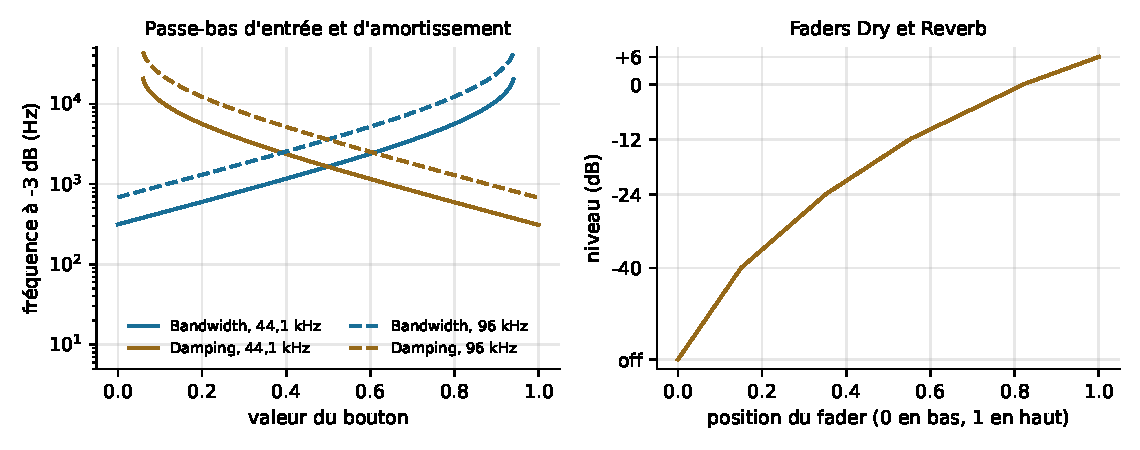
\includegraphics[width=\textwidth]{fig_lois.pdf}
\caption{À gauche : fréquence à $-3$\dB{} des passe-bas Bandwidth et Damping (une courbe
s'arrête quand le filtre reste au-dessus de $-3$\dB{} jusqu'à la fréquence de Nyquist). À
droite : gains du traité et du sec selon Blend.}
\label{fig:lois}
\end{figure}

\paragraph{Fréquence d'échantillonnage.} Les coefficients des filtres ne dépendent pas de $f_s$,
les retards si. À 96\,kHz, Bandwidth et Damping coupent donc deux fois plus haut qu'à 48\,kHz,
comme dans l'original, et le temps de réverbération à une fréquence $f$ est celui qu'on aurait à
$f \times 44\,100/f_s$ à 44,1\,kHz. L'interface affiche les valeurs réelles à la fréquence
courante.

\begin{figure}[htbp]
\centering
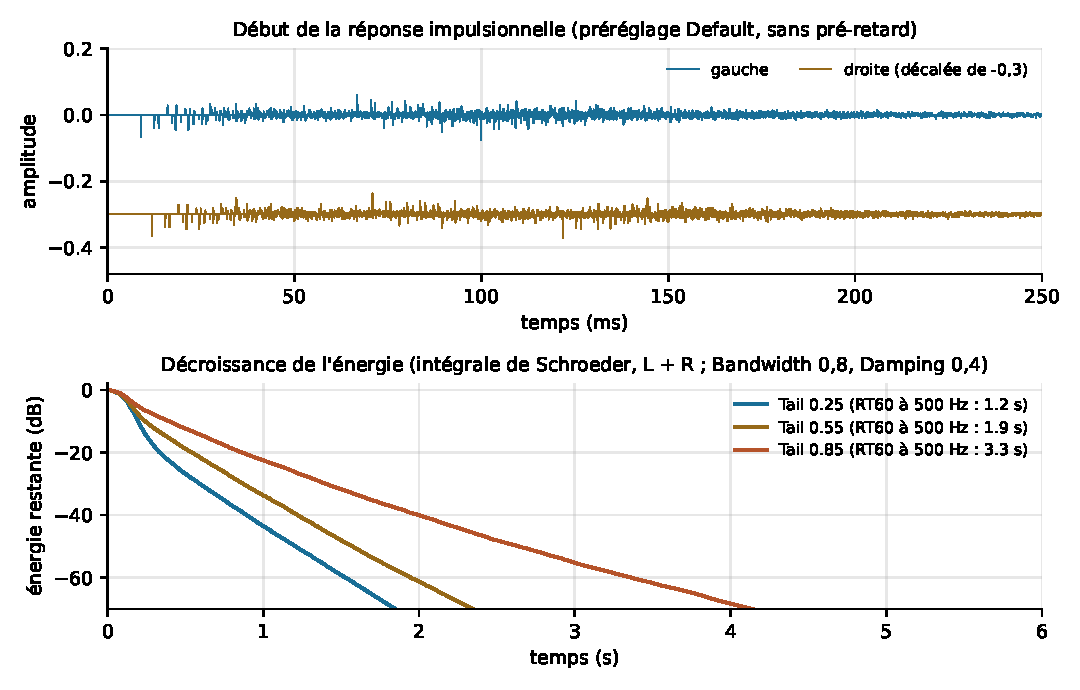
\includegraphics[width=\textwidth]{fig_reponse.pdf}
\caption{En haut : les 250 premières millisecondes de la réponse impulsionnelle de la plaque,
deux canaux. En bas : énergie restante en large bande ; la chute rapide des premiers dixièmes de
seconde vient des aigus, éteints plus tôt par Bandwidth et Damping.}
\label{fig:reponse}
\end{figure}

\subsection{Temps de réverbération}\label{sec:rt60}

Le temps de réverbération (RT60) est le temps que met la réverbération à perdre 60\dB. Le
calculer par le seul gain de boucle (decay$^4$ et deux passages par Damping par tour de 725\,ms)
donne 20 à 60\,\% de moins que la réalité : les passe-tout du réservoir, de coefficients
voisins de 0,72, résonnent d'eux-mêmes (0,5 à 0,65\,s même à Tail 0) et leur retard de groupe
varie avec la fréquence.

L'interface affiche donc des valeurs \textbf{mesurées} : une table de la réponse impulsionnelle
de la plaque à 44,1\,kHz, pour 11 valeurs de Tail, 9 de Damping et 9 bandes d'octave de 62,5\,Hz
à 16\,kHz. Pour chaque point, la réponse (somme des deux canaux) passe par un passe-bande
(Q = 2) ; on intègre son énergie depuis la fin (intégrale de Schroeder) et on prolonge à 60\dB{}
la pente entre $-5$ et $-25$\dB. Entre les points, la table est interpolée linéairement ; une
mesure refaite entre les points de la grille s'écarte de la valeur affichée de moins de 10\,\%
(au plus 7,6\,\% sur les cas vérifiés).

\begin{figure}[htbp]
\centering
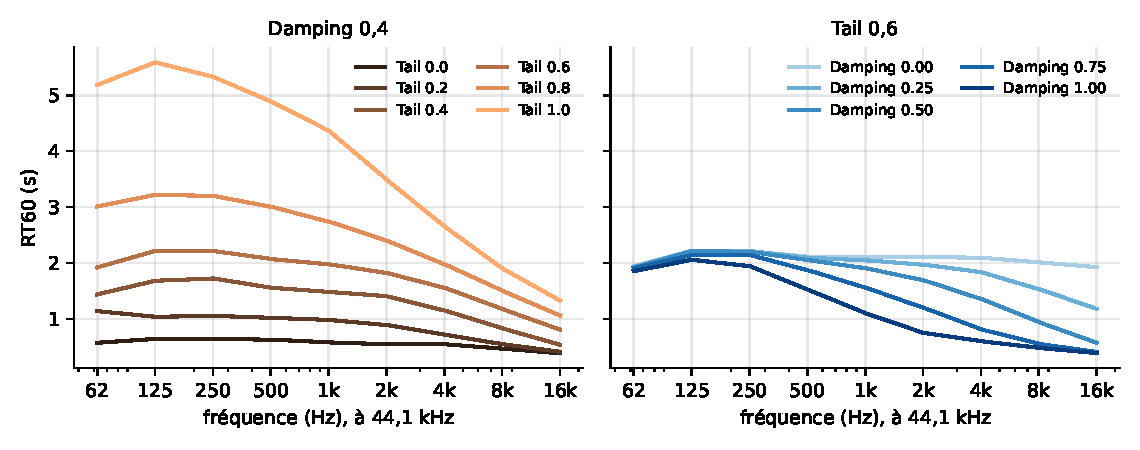
\includegraphics[width=\textwidth]{fig_rt60.pdf}
\caption{Temps de réverbération selon la fréquence (table mesurée, à 44,1\,kHz) : à gauche selon
Tail, à droite selon Damping.}
\label{fig:rt60}
\end{figure}

La figure~\ref{fig:rt60} montre les deux rôles : Tail allonge la réverbération à toutes les
fréquences ; Damping raccourcit surtout l'aigu et laisse le grave presque inchangé.

\subsection{Tonalité : Bandwidth et Low cut}

\paragraph{Low cut.} Passe-haut de Butterworth du second ordre (forme de Robert
Bristow-Johnson, $Q = 1/\sqrt 2$), calculé en double précision, sur les deux canaux de la
réverbération ; sa fréquence est bornée à $0{,}45\,f_s$. À son minimum, ses coefficients sont
ceux de l'identité et il est contourné dès que son état s'est vidé : la sortie est alors exactement
la réverbération non filtrée. La courbe de tonalité de l'interface (figure~\ref{fig:ton}) est le
produit de la réponse de Bandwidth et de celle d'un Butterworth analogique de même fréquence.

\begin{figure}[htbp]
\centering
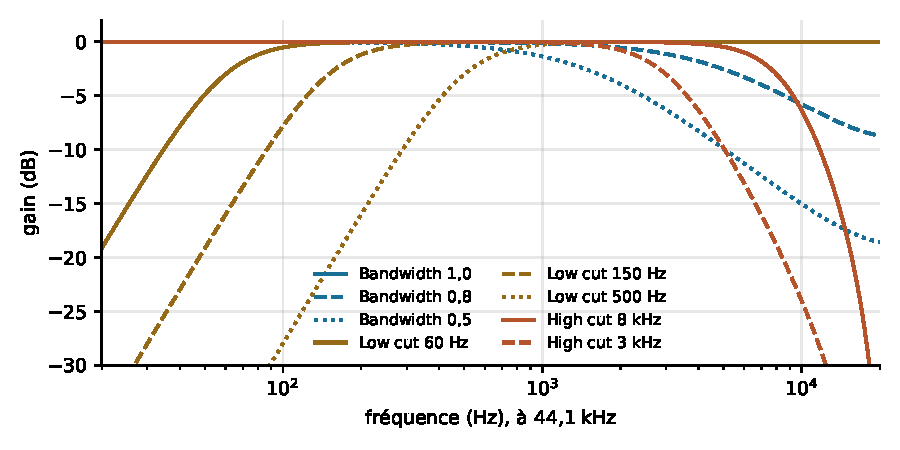
\includegraphics[width=0.75\textwidth]{fig_ton.pdf}
\caption{Réponse du passe-bas d'entrée (Bandwidth) et du coupe-bas de la réverbération (Low
cut), à 44,1\,kHz.}
\label{fig:ton}
\end{figure}

\subsection{Largeur, mélange et sortie}

Avec $m = (w_L + w_R)/2$, $s = (w_L - w_R)/2$ et $W$ la largeur (Width/100) :
\[
w'_L = m + W s, \qquad w'_R = m - W s .
\]
Puis, avec $g_w = \mathrm{blend}^{1{,}53}$ et $G = 10^{\mathrm{Output}/20}$ :
\[
y_{L,R} = \bigl(g_w\, w'_{L,R} + (1 - g_w)\, x_{L,R}\bigr)\, G ,
\]
où $x_{L,R}$ est l'entrée, non retardée : la latence est nulle.

\subsection{Gel (Freeze)}\label{sec:freeze}

Quand Freeze est activé, en 20\,ms : l'entrée de la plaque est fermée, le gain decay va à 1 et
le passe-bas Damping est retiré ; en 200\,ms : la profondeur de la modulation va à 0. La boucle
n'est plus faite que de passe-tout et de retards entiers, qui conservent l'énergie à toutes les
fréquences : le niveau reste constant à $\pm0{,}3$\dB{} sur 20\,s de 100\,Hz à 16\,kHz.

Sans l'arrêt de la modulation, l'interpolation linéaire des retards modulés ferait perdre
l'aigu pendant le gel ($-11$\dB{} à 8\,kHz et $-16$\dB{} à 16\,kHz en 10\,s).

Au relâchement, les mêmes rampes ramènent Tail, Damping, l'entrée et la modulation à leurs
valeurs : la réverbération gelée décroît alors normalement.

\subsection{Lissage des réglages et Bypass}\label{sec:lissage}

L'original applique un changement de réglage au bloc audio suivant, d'un coup : tourner Tail ou
Blend pendant la lecture produit un crépitement (saut de 0,76 sur une sinusoïde d'amplitude
0,5 quand Blend passe de 0 à 1). Ici, chaque coefficient (Bandwidth, decay, Damping, gain
traité, largeur, Output, coefficients du Low cut) va linéairement à sa nouvelle valeur en
20\,ms, puis la prend exactement (même cas : saut de 0,025). Le Pre-delay change par fondu
enchaîné de 30\,ms ; un nouveau changement attend la fin du fondu.

\paragraph{Bypass.} La sortie devient l'entrée, exactement, par un fondu de 10\,ms. La plaque
continue de tourner pendant le Bypass.

\subsection{Identité avec l'original}\label{sec:identite}

Le code de la plaque est une transcription de celui de CAPS 0.9.26 (classes \texttt{PlateStub},
\texttt{Delay}, \texttt{LP1}, \texttt{Sine}) qui garde le type de chaque opération (échantillons
en simple précision, certains produits et sommes en double). Avec Pre-delay 0, Low cut off,
Width 100\,\%, Output 0\dB{} et Freeze inactif (préréglage \og Original (CAPS)\fg, ou n'importe
quelles valeurs des quatre réglages d'origine), la sortie est \textbf{celle de l'original au
bit près}, réglages fixes. C'est vérifié à chaque compilation contre le code source de CAPS
lui-même, appelé comme le ferait un hôte LADSPA : 28 cas (7 réglages à 44,1, 48, 96 et
192\,kHz, blocs de tailles variées), en calcul strict comme avec les options d'optimisation du
greffon.

Quand un réglage bouge, la sortie diffère de l'original par le seul lissage
(section~\ref{sec:lissage}).

\subsection{Nombres dénormaux}

Dans un silence, les états de la plaque décroissent vers zéro et passeraient par les nombres
dénormaux, très lents sur x86. Outre la constante de $\pm 10^{-20}$ de l'original, le greffon
active les modes FTZ/DAZ du processeur le temps de son calcul et rend à l'hôte son propre état
en sortie.

% ==============================================================================================
\section{Conseils d'utilisation}

\begin{description}
\item[Voix.] Vocal plate, ou Pre-delay 30 à 50\,ms pour garder les consonnes devant la
  réverbération ; Low cut 150 à 250\,Hz pour ne pas épaissir le grave.
\item[Batterie.] Drum plate : Tail court, Damping faible pour une queue brillante, Low cut haut.
  Pour une caisse claire très présente, monter Blend plutôt que Tail.
\item[Départ auxiliaire.] Send (100\,\% wet) : Blend à 1, on dose par le niveau du départ. Une
  seule instance pour plusieurs pistes donne un espace commun.
\item[Son sombre et lointain.] Bandwidth bas (moins d'aigus qui entrent), Damping haut (aigus qui
  meurent vite), Tail long : Dark and long.
\item[Largeur.] Width au-delà de 100\,\% élargit la réverbération sans toucher le son direct ;
  vérifier en mono que le mixage ne se creuse pas.
\item[Nappes.] Jouer un accord, activer Freeze, puis jouer par-dessus : l'accord gelé tient sous
  le jeu. Monter Blend pour l'entendre davantage.
\item[Comparer deux réglages.] Régler A, copier vers B (\ctl{A>B}), modifier B, puis basculer A
  | B.
\end{description}

% ==============================================================================================
\section{Fichiers, projets et compatibilité}\label{sec:fichiers}

\begin{description}
\item[Avec le projet.] Tous les réglages et le jeu A/B inactif (état \texttt{ab}). Les réglages
  sont relus par leur nom : ajouter un réglage dans une version future ne casse pas un projet.
\item[Sur l'ordinateur.] Le thème dans \texttt{tinplate.conf} (\texttt{theme=slate} ou
  \texttt{tin}) et vos préréglages dans \texttt{presets/}, un fichier \texttt{<nom>.preset}
  chacun, dans le dossier :
  \begin{itemize}
  \item Windows : \verb|%APPDATA%\Tinplate\| ;
  \item Linux : \verb|$XDG_CONFIG_HOME/tinplate/|, à défaut \verb|~/.config/tinplate/|.
  \end{itemize}
\item[Format d'un préréglage.] Texte, une ligne \texttt{clé=valeur} par réglage
  (\texttt{bandwidth}, \texttt{tail}, \texttt{damping}, \texttt{blend}, \texttt{predelay},
  \texttt{lowcut}, \texttt{width}, \texttt{output}), nombres avec un point décimal quelle que
  soit la langue du système. Une clé absente prend sa valeur par défaut, une valeur hors bornes
  est ramenée dans les bornes, une ligne inconnue est ignorée. Copier le fichier suffit à
  partager un préréglage.
\end{description}

% ==============================================================================================
\section{Limites connues}\label{sec:limites}
\begin{itemize}
\item La taille de la plaque (longueurs des retards) est celle de l'original et ne se règle pas.
\item Bandwidth et Damping coupent plus haut aux fréquences d'échantillonnage élevées
  (comportement de l'original) ; le temps de réverbération change aussi un peu selon la
  fréquence.
\item Le temps de réverbération affiché est une mesure interpolée, juste à 10\,\% près environ.
\item Ce qui est joué pendant le gel n'entre pas dans la réverbération gelée.
\item La saisie au clavier (valeurs, noms de préréglages) dépend de l'hôte : certains gardent le
  clavier pour eux.
\item L'hôte ne voit que les préréglages d'usine.
\end{itemize}

% ==============================================================================================
\section{Crédits}
Algorithme d'origine : Tim Goetze, CAPS, \og C* PlateX2\fg{} (LADSPA, GPL), d'après Jon Dattorro,
\og Effect Design, Part 1: Reverberator and Other Filters\fg, J. Audio Eng. Soc. 45(9), 1997.
Cadre de greffon et interface : DPF (DISTRHO Plugin Framework, ISC). Coupe-bas : formules de
Robert Bristow-Johnson (\emph{Audio EQ Cookbook}).

\end{document}
